\documentclass{standalone}
\usepackage{tikz}
\usetikzlibrary{patterns, positioning}
\usepackage[sfdefault]{ClearSans} %% option 'sfdefault' activates Clear Sans as the default text font
\usepackage[T1]{fontenc}

\begin{document}
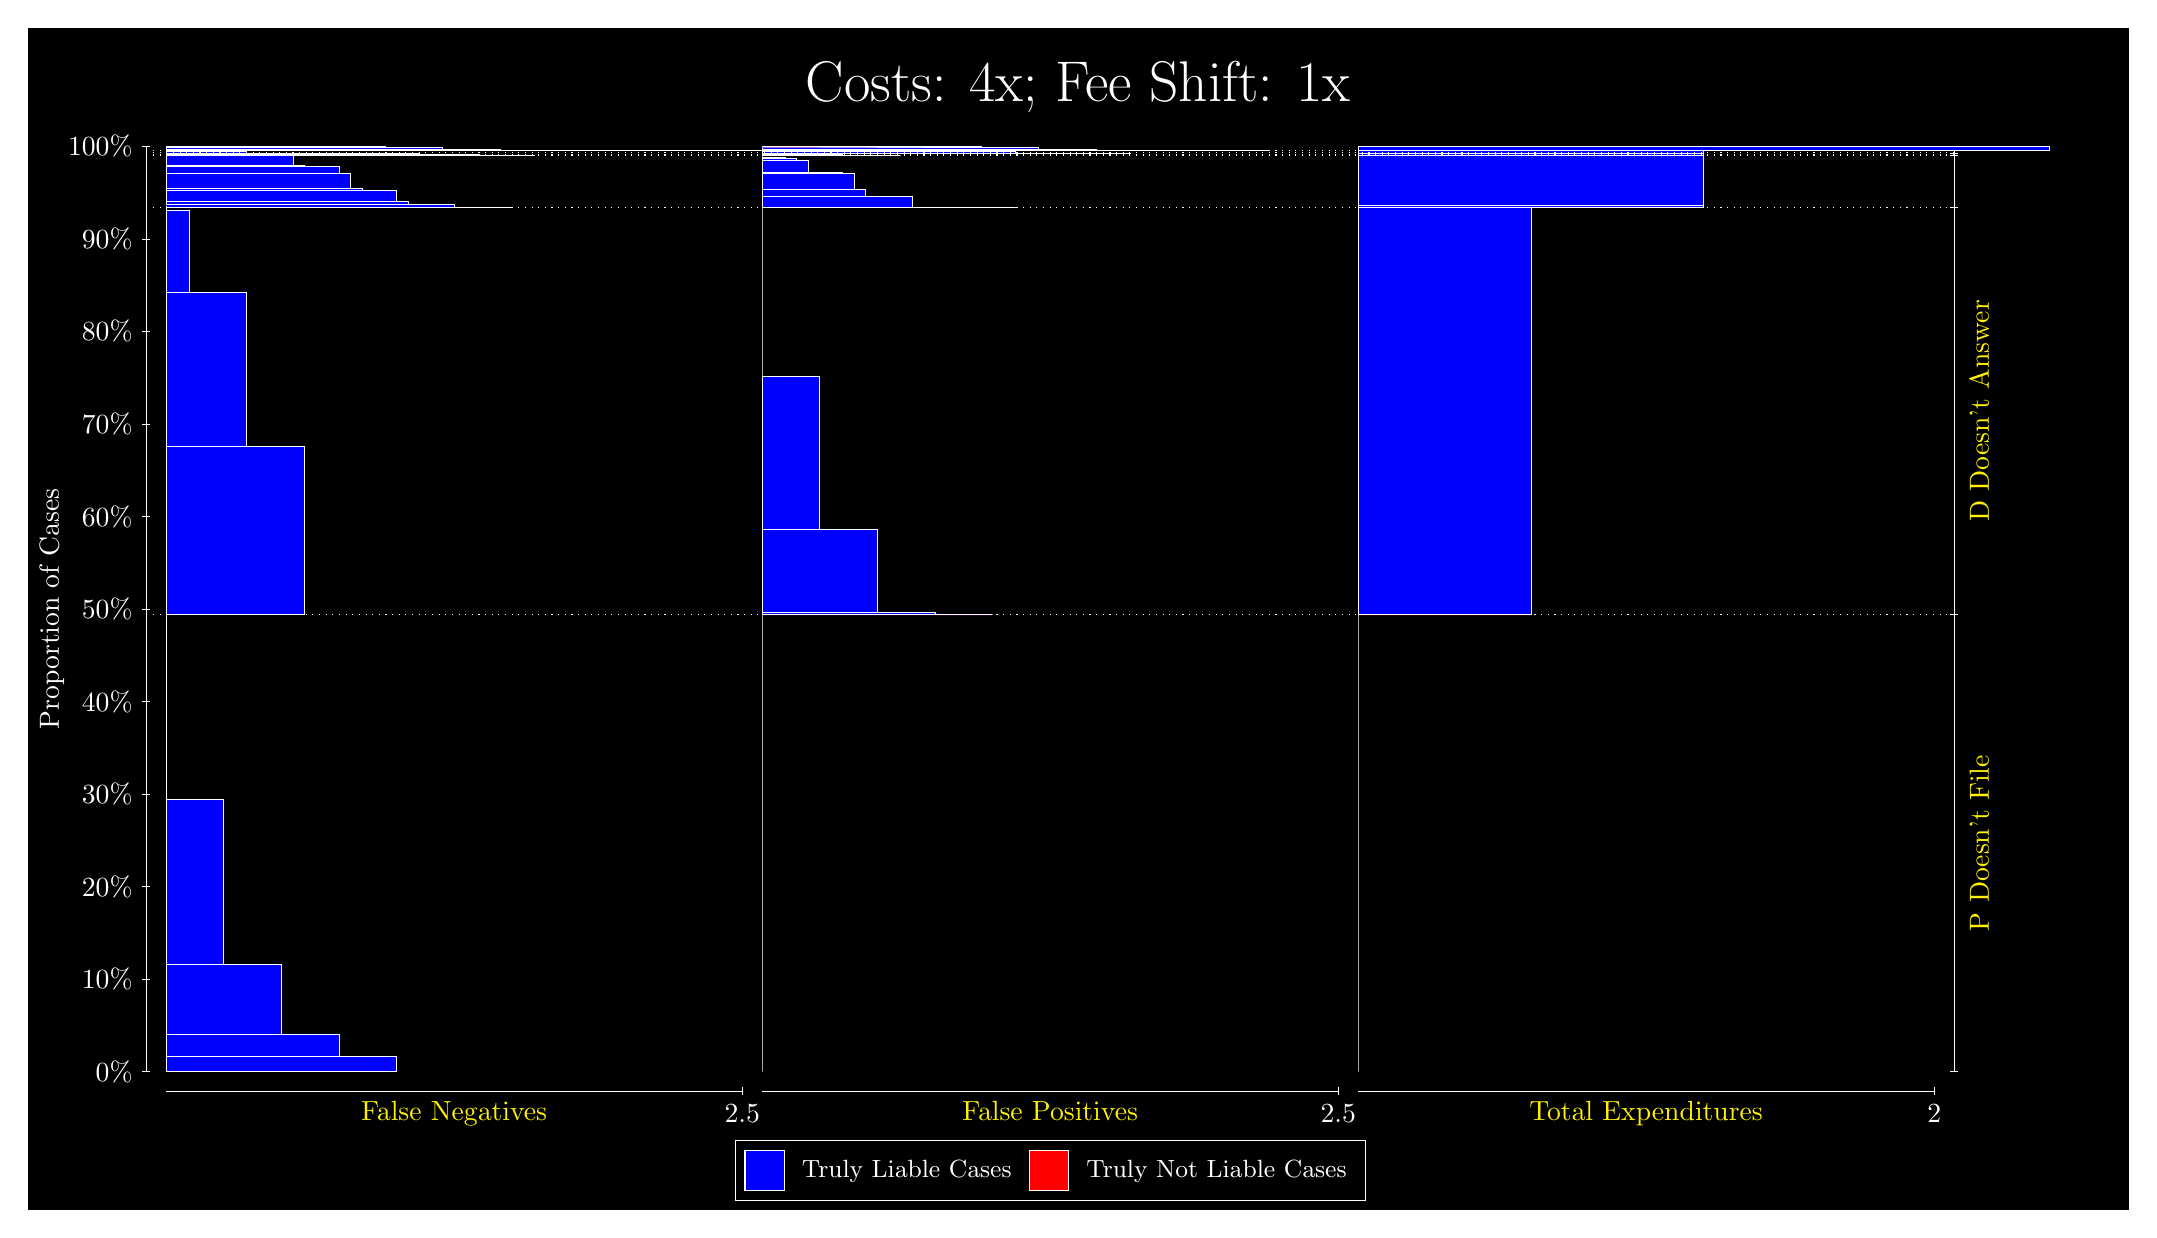
\begin{tikzpicture}
\draw[fill=black] (0,0) rectangle (26.667,15);
\draw[text=white] (0,13.5) rectangle (26.667,15) node[midway] {\huge Costs: 4x; Fee Shift: 1x};
\draw[white, very thin] (1.5,1.75) -- (1.5,13.5);
\node[rotate=90, text=white, anchor=center] at (0.3, 7.625) {Proportion of Cases};
\draw[white, very thin] (1.45,1.75) -- (1.55,1.75);
\node[text=white, anchor=east] at (1.45, 1.75) {0\%};
\draw[white, very thin] (1.45,2.925) -- (1.55,2.925);
\node[text=white, anchor=east] at (1.45, 2.925) {10\%};
\draw[white, very thin] (1.45,4.1) -- (1.55,4.1);
\node[text=white, anchor=east] at (1.45, 4.1) {20\%};
\draw[white, very thin] (1.45,5.275) -- (1.55,5.275);
\node[text=white, anchor=east] at (1.45, 5.275) {30\%};
\draw[white, very thin] (1.45,6.45) -- (1.55,6.45);
\node[text=white, anchor=east] at (1.45, 6.45) {40\%};
\draw[white, very thin] (1.45,7.625) -- (1.55,7.625);
\node[text=white, anchor=east] at (1.45, 7.625) {50\%};
\draw[white, very thin] (1.45,8.8) -- (1.55,8.8);
\node[text=white, anchor=east] at (1.45, 8.8) {60\%};
\draw[white, very thin] (1.45,9.975) -- (1.55,9.975);
\node[text=white, anchor=east] at (1.45, 9.975) {70\%};
\draw[white, very thin] (1.45,11.15) -- (1.55,11.15);
\node[text=white, anchor=east] at (1.45, 11.15) {80\%};
\draw[white, very thin] (1.45,12.325) -- (1.55,12.325);
\node[text=white, anchor=east] at (1.45, 12.325) {90\%};
\draw[white, very thin] (1.45,13.5) -- (1.55,13.5);
\node[text=white, anchor=east] at (1.45, 13.5) {100\%};

\draw[white, very thin] (24.457,1.75) -- (24.457,13.5);
\draw[white, very thin] (24.407,1.75) -- (24.507,1.75);
\node[anchor=west] at (24.407, 1.75) {};
\draw[white, very thin] (24.407,7.5517) -- (24.507,7.5517);
\node[anchor=west] at (24.407, 7.5517) {};
\draw[white, very thin] (24.407,12.728) -- (24.507,12.728);
\node[anchor=west] at (24.407, 12.728) {};
\draw[white, very thin] (24.407,13.39) -- (24.507,13.39);
\node[anchor=west] at (24.407, 13.39) {};
\draw[white, very thin] (24.407,13.418) -- (24.507,13.418);
\node[anchor=west] at (24.407, 13.418) {};
\draw[white, very thin] (24.407,13.451) -- (24.507,13.451);
\node[anchor=west] at (24.407, 13.451) {};
\draw[white, very thin] (24.407,13.5) -- (24.507,13.5);
\node[anchor=west] at (24.407, 13.5) {};

\draw[white, very thin, fill=blue] (1.75,1.75) rectangle (4.6775,1.9467);
\draw[white, very thin, fill=blue] (1.75,1.9467) rectangle (3.9457,2.2265);
\draw[white, very thin, fill=blue] (1.75,2.2265) rectangle (3.2138,3.1154);
\draw[white, very thin, fill=blue] (1.75,3.1154) rectangle (2.4819,5.2043);
\draw[white, very thin, fill=red] (1.75,5.2043) rectangle (1.75,5.2043);
\draw[white, very thin, fill=blue] (1.75,5.2043) rectangle (1.75,7.5517);
\draw[white, very thin, fill=blue] (1.75,7.5517) rectangle (3.5065,9.6954);
\draw[white, very thin, fill=blue] (1.75,9.6954) rectangle (2.7746,11.642);
\draw[white, very thin, fill=blue] (1.75,11.642) rectangle (2.0428,12.692);
\draw[white, very thin, fill=red] (1.75,12.692) rectangle (1.75,12.692);
\draw[white, very thin, fill=blue] (1.75,12.692) rectangle (1.75,12.728);
\draw[white, very thin, fill=blue] (1.75,12.728) rectangle (6.1413,12.728);
\draw[white, very thin, fill=blue] (1.75,12.728) rectangle (5.8486,12.728);
\draw[white, very thin, fill=blue] (1.75,12.728) rectangle (5.5558,12.729);
\draw[white, very thin, fill=blue] (1.75,12.729) rectangle (5.4094,12.759);
\draw[white, very thin, fill=blue] (1.75,12.759) rectangle (5.2631,12.759);
\draw[white, very thin, fill=blue] (1.75,12.759) rectangle (5.1167,12.76);
\draw[white, very thin, fill=blue] (1.75,12.76) rectangle (4.9703,12.767);
\draw[white, very thin, fill=blue] (1.75,12.767) rectangle (4.8239,12.801);
\draw[white, very thin, fill=blue] (1.75,12.801) rectangle (4.6775,12.944);
\draw[white, very thin, fill=blue] (1.75,12.944) rectangle (4.5312,12.945);
\draw[white, very thin, fill=blue] (1.75,12.945) rectangle (4.3848,12.948);
\draw[white, very thin, fill=blue] (1.75,12.948) rectangle (4.2384,12.963);
\draw[white, very thin, fill=blue] (1.75,12.963) rectangle (4.092,13.163);
\draw[white, very thin, fill=blue] (1.75,13.163) rectangle (3.9457,13.249);
\draw[white, very thin, fill=blue] (1.75,13.249) rectangle (3.7993,13.25);
\draw[white, very thin, fill=blue] (1.75,13.25) rectangle (3.6529,13.25);
\draw[white, very thin, fill=blue] (1.75,13.25) rectangle (3.5065,13.254);
\draw[white, very thin, fill=blue] (1.75,13.254) rectangle (3.3602,13.387);
\draw[white, very thin, fill=blue] (1.75,13.387) rectangle (3.2138,13.388);
\draw[white, very thin, fill=blue] (1.75,13.388) rectangle (3.0674,13.388);
\draw[white, very thin, fill=blue] (1.75,13.388) rectangle (2.921,13.388);
\draw[white, very thin, fill=blue] (1.75,13.388) rectangle (2.7746,13.388);
\draw[white, very thin, fill=blue] (1.75,13.388) rectangle (2.6283,13.39);
\draw[white, very thin, fill=blue] (1.75,13.39) rectangle (2.3355,13.39);
\draw[white, very thin, fill=blue] (1.75,13.39) rectangle (2.0428,13.39);
\draw[white, very thin, fill=red] (1.75,13.39) rectangle (1.75,13.39);
\draw[white, very thin, fill=blue] (1.75,13.39) rectangle (6.4341,13.39);
\draw[white, very thin, fill=blue] (1.75,13.39) rectangle (5.7022,13.399);
\draw[white, very thin, fill=blue] (1.75,13.399) rectangle (4.9703,13.414);
\draw[white, very thin, fill=blue] (1.75,13.414) rectangle (4.2384,13.418);
\draw[white, very thin, fill=blue] (1.75,13.418) rectangle (3.5065,13.418);
\draw[white, very thin, fill=red] (1.75,13.418) rectangle (1.75,13.418);
\draw[white, very thin, fill=blue] (1.75,13.418) rectangle (3.5065,13.418);
\draw[white, very thin, fill=blue] (1.75,13.418) rectangle (2.7746,13.437);
\draw[white, very thin, fill=blue] (1.75,13.437) rectangle (2.0428,13.451);
\draw[white, very thin, fill=red] (1.75,13.451) rectangle (1.75,13.451);
\draw[white, very thin, fill=blue] (1.75,13.451) rectangle (1.75,13.451);
\draw[white, very thin, fill=blue] (1.75,13.451) rectangle (11.704,13.451);
\draw[white, very thin, fill=blue] (1.75,13.451) rectangle (10.972,13.451);
\draw[white, very thin, fill=blue] (1.75,13.451) rectangle (10.24,13.452);
\draw[white, very thin, fill=blue] (1.75,13.452) rectangle (9.508,13.455);
\draw[white, very thin, fill=blue] (1.75,13.455) rectangle (8.7761,13.455);
\draw[white, very thin, fill=blue] (1.75,13.455) rectangle (8.0442,13.455);
\draw[white, very thin, fill=blue] (1.75,13.455) rectangle (7.4587,13.455);
\draw[white, very thin, fill=blue] (1.75,13.455) rectangle (7.3123,13.455);
\draw[white, very thin, fill=blue] (1.75,13.455) rectangle (6.7268,13.455);
\draw[white, very thin, fill=blue] (1.75,13.455) rectangle (5.9949,13.464);
\draw[white, very thin, fill=blue] (1.75,13.464) rectangle (5.2631,13.488);
\draw[white, very thin, fill=blue] (1.75,13.488) rectangle (4.5312,13.499);
\draw[white, very thin, fill=blue] (1.75,13.499) rectangle (3.7993,13.5);
\draw[white, very thin, fill=blue] (1.75,13.5) rectangle (3.0674,13.5);
\draw[white, very thin, fill=blue] (1.75,13.5) rectangle (2.3355,13.5);
\draw[white, very thin, fill=red] (1.75,13.5) rectangle (1.75,13.5);
\draw[white, very thin, fill=red] (9.3189,1.75) rectangle (9.3189,1.75);
\draw[white, very thin, fill=blue] (9.3189,1.75) rectangle (9.3189,7.5517);
\draw[white, very thin, fill=red] (9.3189,7.5517) rectangle (12.246,7.5517);
\draw[white, very thin, fill=blue] (9.3189,7.5517) rectangle (12.246,7.5517);
\draw[white, very thin, fill=blue] (9.3189,7.5517) rectangle (11.515,7.5874);
\draw[white, very thin, fill=blue] (9.3189,7.5874) rectangle (10.783,8.6373);
\draw[white, very thin, fill=blue] (9.3189,8.6373) rectangle (10.051,10.584);
\draw[white, very thin, fill=blue] (9.3189,10.584) rectangle (9.3189,12.728);
\draw[white, very thin, fill=red] (9.3189,12.728) rectangle (12.539,12.728);
\draw[white, very thin, fill=blue] (9.3189,12.728) rectangle (12.539,12.728);
\draw[white, very thin, fill=red] (9.3189,12.728) rectangle (12.246,12.728);
\draw[white, very thin, fill=blue] (9.3189,12.728) rectangle (12.246,12.728);
\draw[white, very thin, fill=red] (9.3189,12.728) rectangle (11.954,12.728);
\draw[white, very thin, fill=blue] (9.3189,12.728) rectangle (11.954,12.73);
\draw[white, very thin, fill=blue] (9.3189,12.73) rectangle (11.807,12.73);
\draw[white, very thin, fill=red] (9.3189,12.73) rectangle (11.661,12.73);
\draw[white, very thin, fill=blue] (9.3189,12.73) rectangle (11.661,12.73);
\draw[white, very thin, fill=blue] (9.3189,12.73) rectangle (11.515,12.73);
\draw[white, very thin, fill=red] (9.3189,12.73) rectangle (11.368,12.73);
\draw[white, very thin, fill=blue] (9.3189,12.73) rectangle (11.368,12.731);
\draw[white, very thin, fill=blue] (9.3189,12.731) rectangle (11.222,12.864);
\draw[white, very thin, fill=blue] (9.3189,12.864) rectangle (11.075,12.868);
\draw[white, very thin, fill=blue] (9.3189,12.868) rectangle (10.929,12.868);
\draw[white, very thin, fill=blue] (9.3189,12.868) rectangle (10.783,12.869);
\draw[white, very thin, fill=blue] (9.3189,12.869) rectangle (10.636,12.955);
\draw[white, very thin, fill=blue] (9.3189,12.955) rectangle (10.49,13.155);
\draw[white, very thin, fill=blue] (9.3189,13.155) rectangle (10.344,13.17);
\draw[white, very thin, fill=blue] (9.3189,13.17) rectangle (10.197,13.173);
\draw[white, very thin, fill=blue] (9.3189,13.173) rectangle (10.051,13.174);
\draw[white, very thin, fill=blue] (9.3189,13.174) rectangle (9.9044,13.317);
\draw[white, very thin, fill=blue] (9.3189,13.317) rectangle (9.758,13.351);
\draw[white, very thin, fill=blue] (9.3189,13.351) rectangle (9.6116,13.358);
\draw[white, very thin, fill=blue] (9.3189,13.358) rectangle (9.4652,13.359);
\draw[white, very thin, fill=blue] (9.3189,13.359) rectangle (9.3189,13.39);
\draw[white, very thin, fill=red] (9.3189,13.39) rectangle (11.075,13.39);
\draw[white, very thin, fill=blue] (9.3189,13.39) rectangle (11.075,13.39);
\draw[white, very thin, fill=blue] (9.3189,13.39) rectangle (10.344,13.394);
\draw[white, very thin, fill=blue] (9.3189,13.394) rectangle (9.6116,13.409);
\draw[white, very thin, fill=blue] (9.3189,13.409) rectangle (9.3189,13.418);
\draw[white, very thin, fill=red] (9.3189,13.418) rectangle (14.003,13.418);
\draw[white, very thin, fill=blue] (9.3189,13.418) rectangle (14.003,13.418);
\draw[white, very thin, fill=blue] (9.3189,13.418) rectangle (13.271,13.418);
\draw[white, very thin, fill=blue] (9.3189,13.418) rectangle (12.539,13.432);
\draw[white, very thin, fill=blue] (9.3189,13.432) rectangle (11.807,13.451);
\draw[white, very thin, fill=blue] (9.3189,13.451) rectangle (11.075,13.451);
\draw[white, very thin, fill=red] (9.3189,13.451) rectangle (15.759,13.451);
\draw[white, very thin, fill=blue] (9.3189,13.451) rectangle (15.759,13.451);
\draw[white, very thin, fill=blue] (9.3189,13.451) rectangle (15.028,13.451);
\draw[white, very thin, fill=red] (9.3189,13.451) rectangle (15.028,13.451);
\draw[white, very thin, fill=blue] (9.3189,13.451) rectangle (15.028,13.451);
\draw[white, very thin, fill=blue] (9.3189,13.451) rectangle (14.296,13.452);
\draw[white, very thin, fill=red] (9.3189,13.452) rectangle (14.296,13.452);
\draw[white, very thin, fill=blue] (9.3189,13.452) rectangle (14.296,13.452);
\draw[white, very thin, fill=blue] (9.3189,13.452) rectangle (13.564,13.456);
\draw[white, very thin, fill=red] (9.3189,13.456) rectangle (13.564,13.456);
\draw[white, very thin, fill=blue] (9.3189,13.456) rectangle (13.564,13.463);
\draw[white, very thin, fill=blue] (9.3189,13.463) rectangle (12.832,13.464);
\draw[white, very thin, fill=blue] (9.3189,13.464) rectangle (12.832,13.487);
\draw[white, very thin, fill=blue] (9.3189,13.487) rectangle (12.1,13.496);
\draw[white, very thin, fill=blue] (9.3189,13.496) rectangle (11.368,13.496);
\draw[white, very thin, fill=red] (9.3189,13.496) rectangle (10.783,13.496);
\draw[white, very thin, fill=blue] (9.3189,13.496) rectangle (10.783,13.496);
\draw[white, very thin, fill=blue] (9.3189,13.496) rectangle (10.636,13.496);
\draw[white, very thin, fill=red] (9.3189,13.496) rectangle (10.051,13.496);
\draw[white, very thin, fill=blue] (9.3189,13.496) rectangle (10.051,13.496);
\draw[white, very thin, fill=red] (9.3189,13.496) rectangle (9.3189,13.496);
\draw[white, very thin, fill=blue] (9.3189,13.496) rectangle (9.3189,13.5);
\draw[white, very thin, fill=red] (16.888,1.75) rectangle (16.888,1.75);
\draw[white, very thin, fill=blue] (16.888,1.75) rectangle (16.888,7.5517);
\draw[white, very thin, fill=red] (16.888,7.5517) rectangle (19.083,7.5517);
\draw[white, very thin, fill=blue] (16.888,7.5517) rectangle (19.083,12.728);
\draw[white, very thin, fill=red] (16.888,12.728) rectangle (21.279,12.728);
\draw[white, very thin, fill=blue] (16.888,12.728) rectangle (21.279,12.754);
\draw[white, very thin, fill=red] (16.888,12.754) rectangle (21.279,12.754);
\draw[white, very thin, fill=blue] (16.888,12.754) rectangle (21.279,13.39);
\draw[white, very thin, fill=red] (16.888,13.39) rectangle (21.279,13.39);
\draw[white, very thin, fill=blue] (16.888,13.39) rectangle (21.279,13.418);
\draw[white, very thin, fill=red] (16.888,13.418) rectangle (21.279,13.418);
\draw[white, very thin, fill=blue] (16.888,13.418) rectangle (21.279,13.451);
\draw[white, very thin, fill=red] (16.888,13.451) rectangle (25.67,13.451);
\draw[white, very thin, fill=blue] (16.888,13.451) rectangle (25.67,13.456);
\draw[white, very thin, fill=red] (16.888,13.456) rectangle (25.67,13.456);
\draw[white, very thin, fill=blue] (16.888,13.456) rectangle (25.67,13.5);
\draw[white, dotted] (1.5,7.5517) -- (24.457,7.5517);
\draw[white, dotted] (1.5,12.728) -- (24.457,12.728);
\draw[white, dotted] (1.5,13.39) -- (24.457,13.39);
\draw[white, dotted] (1.5,13.418) -- (24.457,13.418);
\draw[white, dotted] (1.5,13.451) -- (24.457,13.451);
\draw[white, very thin] (1.75,1.5) -- (9.0689,1.5);
\node[text=yellow, anchor=north] at (5.4094, 1.5) {False Negatives};
\draw[white, very thin] (9.0689,1.45) -- (9.0689,1.55);
\node[text=white, anchor=north] at (9.0689, 1.45) {2.5};

\draw[white, very thin] (9.3189,1.5) -- (16.638,1.5);
\node[text=yellow, anchor=north] at (12.978, 1.5) {False Positives};
\draw[white, very thin] (16.638,1.45) -- (16.638,1.55);
\node[text=white, anchor=north] at (16.638, 1.45) {2.5};

\draw[white, very thin] (16.888,1.5) -- (24.207,1.5);
\node[text=yellow, anchor=north] at (20.547, 1.5) {Total Expenditures};
\draw[white, very thin] (24.207,1.45) -- (24.207,1.55);
\node[text=white, anchor=north] at (24.207, 1.45) {2};

\node[text=yellow, centered, rotate=90] at (24.777, 4.6508) {P Doesn't File};
\node[text=yellow, centered, rotate=90] at (24.777, 10.14) {D Doesn't Answer};





\draw (12.978300999999998,1.5) node[draw=none] (baseCoordinate) {};
\begin{scope}[align=center]
        \matrix[scale=0.5, draw=white, below=0.5cm of baseCoordinate, nodes={draw}, column sep=0.1cm]{
            \node[rectangle, draw, minimum width=0.5cm, minimum height=0.5cm, fill=blue] {}; &
            \node[draw=none, font=\small, text=white] (B) {Truly Liable Cases}; &
            \node[rectangle, draw, minimum width=0.5cm, minimum height=0.5cm, fill=red] {}; &
            \node[draw=none, font=\small, text=white] (B) {Truly Not Liable Cases}; \\
            };
\end{scope}

\end{tikzpicture}
\end{document}